\section{Proposed Approach}
% Delete the text and write your Method(s) here:
%------------------------------------
\subsection{Motivation}
Of all the papers that we examined, we were interested in the work done by Bhushan and Lee \cite{bhushan-lee-2022-block} on block diagram summarization capabilities. Although Blosum performed respectably well for the online generated block diagrams, it struggles mainly with hand-written texts. This was due to the version of EasyOCR not supporting handwritten texts and the focus of Blosum being on computerized block diagrams. Hence, our project would focus on improving the Blosum architecture to better detect handwritten text, to generate a better performance on the $FC\_A$ dataset. \par

Based on this, our project centers around modifying the existing architecture presented by Bhushan and Lee \cite{bhushan-lee-2022-block} to better detect handwritten block diagrams. Blosum is comprised of mainly four parts, as shown in the \Cref{fig:Blosum architure}. It consists of shape prediction, text prediction, arrow prediction and triplet generation. We propose that by experimenting with the backbone of the Blosum architecture, we may be able to derive better results with regards to the shape prediction, leading to a better performance on the $FC\_A$ dataset. 

\begin{figure}
    \centering
    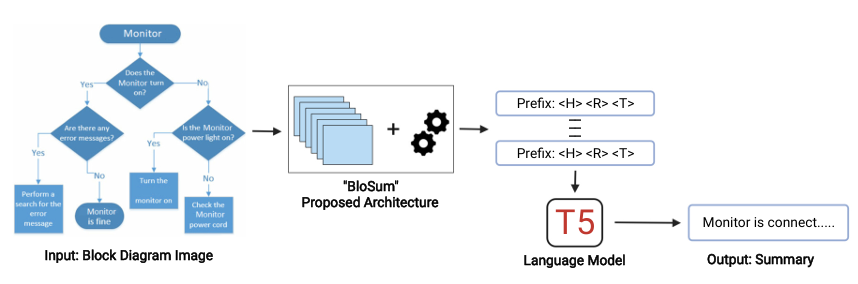
\includegraphics[width=0.48\textwidth]{Images/Blosum architecture.png}
    \caption{Blosum architecture proposed by Bhushan and Lee \cite{bhushan-lee-2022-block}.}
    \label{fig:Blosum architure}
\end{figure}


\subsection{Our Model}
Our architecture model explored in this project followed the architecture used Bhushan and Lee \cite{bhushan-lee-2022-block}. Focusing on the shape prediction portion, we substituted the Inception-ResNet-v2 backbone for a Swin transformer instead. 

The choice of the Swin transformer was due to its ability to deal with small visual entities and pixel level patterns. The Swin transformer can address these challenges by proposing hierarchical processing of image tokens using shifted window patches with linear complexity to image size \cite{singh_2024_swin}.  This hierarchical architecture has the flexibility to model at various scales and has linear computational complexity with respect to image size \cite{liu_2021_swin}, allowing greater performance when detecting arrowheads in block diagrams.


\subsection{Shape Prediction and Triplet Generation}
The shape prediction feature was treated as an object detection task. Similar to Bhushan and Lee \cite{bhushan-lee-2022-block}, for each shape $s \in S$, it predicts a bounding box $bs \in R4$ and a class name $cs \in C$. We defined seven plus one (background) different classes, which include Connection, Data, Decision, Terminator, and Process. 

The Inception-ResNet-v2 backbone here worked by having multi-level feature extraction that can capture information at various scales and complexities. Dimensionality reduction and pooling was also carried out to reduce the complexity and reduce over fitting respectively. To ensure fair testing, we also kept the similar intersection over union (IoU) threshold value of 0.8 over all shape classes. To prevent duplicates, a non-maximum suppression (NMS) was applied. 


Additionally, based on the information collected from the previous steps, we created a similar pipeline used to form a triplet generator. The generator would capture the relationship between the shapes detected by finding the closest anchor point placed on other shapes.

